\documentclass[aps,prd,reprint,nofootinbib, superscriptaddress]{revtex4-1}
\usepackage{amsmath,amssymb, amsthm,amstext}
\usepackage{natbib}
\usepackage{graphicx}
\usepackage{color}
\usepackage{array, enumerate}
\usepackage{bm}
\usepackage{multirow}
\usepackage[breaklinks,colorlinks,citecolor=blue]{hyperref}


% Shorts
\def\nn{\nonumber}
\def\st{\sin\theta}
\def\ct{\cos\theta}
\def\sst{\sin^2\theta}
\def\cct{\cos^2\theta}
\def\Ap{A_\phi}
\def\Ar{A_{\phi,r}}
\def\Arr{A_{\phi,rr}}
\def\Am{A_{\phi,\mu}}
\def\Amm{A_{\phi,\mu\mu}}
\def\Ah{A_{\phi,\theta}}
\def\be{\begin{equation}}
\def\ee{\end{equation}}
\def\ben{\begin{eqnarray}}
\def\een{\end{eqnarray}}
\def\WH{\Omega_{\rm H}}
\def\e{{\bf e}}
\def\AHE{A_\phi^{\rm HE}}
\def\AEE{A_\phi^{\rm EE}}


\def\Alfven{Alfv\`en}


\begin{document}
\title{The force-free magnetosphere of a Kerr black hole: the role of boundary conditions}
\author{Zhen Pan}
\email{zpan@perimeterinstitute.ca}
\affiliation{Perimeter Institute for Theoretical Physics, Waterloo, Ontario N2L 2Y5, Canada}

\date{\today}

\begin{abstract}
    The role of boundary conditions in the structure of
    a force-free black hole magnetosphere was rarely discussed, since previous studies have been focused on the
    the field lines entering the horizon which is causally disconnected and on which the boundary
    condition imposed usually makes no difference to the magnetosphere structure. However,
    recent high-resolution general relativistic (GR) force-free simulation shows that there are both
    field lines entering the horizon and field lines ending up on the equatorial current sheet
    within the ergosphere for asymptotic uniform field. For the latter, the equatorial boundary
    condition is well approximated being marginally force-free, i.e., $B^2-E^2=0$, where $B$ and
    $E$ are the magnetic and electric field strength, respectively. In this paper, we revisit this
    problem by solving the GR Grad-Shafranov equation which governs the structure of
    the force-free magnetosphere in steady state and self-consistently imposing the marginally force-free equatorial
    condition. We also discuss the applicability of this boundary condition and the numerical algorithm proposed
    in this paper for general magnetic field configurations.
\end{abstract}


\maketitle

\section{Introduction}

The paper is organized as follows.  In Section \ref{sec:basic}, we outline the basic governing equations.
In Section \ref{sec:uni_sol}, we clarify the radiation condition, boundary conditions and numerical algorithm
for the uniform field solution. In Section \ref{sec:discussion}, we discuss the solution uniqueness, near-horizon
field line configuration and the application to general field line configurations. Summary is given in Section \ref{sec:summary}.


\section{basic equations}
\label{sec:basic}
In this paper, we adopt the Kerr-Schild
coordinate with the line element
\[
\begin{aligned}
ds^2 =
&-\left( 1-\frac{2r}{\Sigma} \right)dt^2 + \left( \frac{4
r}{\Sigma} \right) dr dt + \left(1+\frac{2r}{\Sigma} \right) dr^2 \\
&+ \Sigma d\theta^2 - \frac{4 a r \sin^2\theta}{\Sigma} d\phi dt
- 2 a \left(1+\frac{2r}{\Sigma}\right) \sin^2\theta d\phi dr     \\
& + \frac{\beta}{\Sigma} \sst d\phi^2
\end{aligned}
\]
where $\Sigma = r^2 + a^2 \mu^2$, $\Delta = r^2 -2r + a^2$,
$\beta = \Delta\Sigma + 2r(r^2 + a^2)$, and $a$ is the dimensionless BH spin.
In the force-free approximation, electromagnetic energy greatly exceeds that of matter.
Consequently, the force-free magnetospheres is governed by energy
conservation equation of electromagnetic field, or
conventionally called as the GS equation.
In the Kerr spacetime,
the axisymmetric and steady GS equation can be written in a compact form \cite{Pan2017}
\ben
\label{eq:GSg}
&&\phantom{+}
 \left[\Arr + \frac{\sst}{\Delta}\Amm \right]  \mathcal K(r,\theta; \Omega )\nn \\
&&
+\left[\Ar \partial_r^\Omega  +  \frac{\sst}{\Delta}\Am \partial_\mu^\Omega\right] \mathcal K(r,\theta; \Omega ) \nn \\
&&
+ \frac{1}{2}\left[\Ar^2 + \frac{\sst}{\Delta}\Am^2\right]  \Omega' \partial_\Omega \mathcal K(r,\theta; \Omega )\nn \\
&&
- \frac{\Sigma}{\Delta}II' = 0 \ ,
\een
with $\mathcal K(r,\theta; \Omega )= \left[\frac{\beta}{\Sigma}\Omega^2 \sst
-\frac{4ra}{\Sigma}\Omega \sst
-\left(1-\frac{2r}{\Sigma}\right)\right]$ being the LS function,
$\mu\equiv\ct$,  and  the primes designate  derivatives with respect to $A_\phi$.
$\partial_i^\Omega (i=r, \mu)$  denotes the partial derivative
with respect to coordinate $i$ with $\Omega$ fixed, and $\partial_\Omega$ is the derivative with
respect to $\Omega$.

\section{Uniform field solution}
\label{sec:uni_sol}

\subsection{Solution uniqueness and radiation condition}
For common field configurations, including split monopole and parabola, there exist two LSs where
the LS function vanishes and the GS equation degrades from second order to first order. As proposed
by Contopoulos et.al. \cite{Contopoulos2013}, one can adjust the two free functions $\Omega(\Ap)$
and $I(\Ap)$ enabling field lines smoothly cross the two LSs, then the solution
$\{\Omega(\Ap), I(\Ap), \Ap(r,\theta)\}$  is uniquely found. But for the vertical field lines, their
exist only one LS, which is insufficient to determine two free functions. Therefore people have been
wondering the possibility of many solutions though the many-solutions scenario is not supported by force-free
dynamics simulations. To tackle this problem, we proposed that the two functions are not independent;
instead, they are related by the radiation condition \cite{Pan2016a, Pan2017}
\be I = 2\Omega A_\phi, \label{eq:rad}\ee
which has been confirmed by the recent high-accuracy simulations \cite{East2018}.

\subsection{Boundary conditions}

The boundary conditions at infinity (inner infinity $r=r_+$ and outer infinity $r\rightarrow\infty$)
and on the polar axis can be simply set as
\be
\begin{aligned}
\Ar|_{r=r_+, \infty} &= 0, \\
A_\phi|_{\mu = 1} &= 0,\\
\end{aligned}
\ee
where $r_+$ is the radius of the event horizon,
while the equatorial boundary conditions are more unclear until recent simulations \cite{East2018}
come out which show that there exists an equator current sheet within the ergosphere where the
magnetic dominance marginally loses, i.e., $B^2-E^2\approx 0$. Motivated by these simulations,
we choose the following equatorial boundary condition in our numerical solutions,
\begin{subequations}
\begin{align}
    \Am(\mu = 0, r > 2) &= 0, \label{eq:bc2}\\
    B^2-E^2 (\mu = 0, r_+ \leq r \leq 2) &=0.\label{eq:bc3}
\end{align}
\end{subequations}
In fact, Equation (\ref{eq:bc3})
is neither a Dirichlet nor a Neumann boundary condition, since
\be
\begin{aligned}
&B^2-E^2 \\
= & \frac{1}{\Sigma \sst} \left[ -\mathcal{K} \left(\Ar^2 +\frac{\sst}{\Delta}\Am^2 \right)+\frac{\Sigma}{\Delta}I^2\right],
\end{aligned}
\ee
which involves both derivatives $\Am$ and $\Ar$ on the boundary.
Therefore, it is numerically non-trivial to impose this boundary condition in computation.

In addition, there is a coordinate singularity $1/\Delta$ in the expression of $B^2-E^2$.
To avoid possible numerical difficulty, we use the prescription
\be
\label{eq:nbc}
\int_{A_\phi^{\rm HE}}^{A_\phi^{\rm EE}} \left(\frac{B^2-E^2}{B^2+E^2}\right)^2 dA_\phi \Bigg/ \left(A_\phi^{\rm EE}- A_\phi^{\rm HE}\right)  < 10^{-3},
\ee
in our computation, as a proxy of the marginally force-free equatorial boundary condition (\ref{eq:bc3}),
where $\AHE$ and $\AEE$ are the magnetic flux entering the horizon and the ergosphere, respectively;
``HE" and ``EE" are short for Horizon-Equator and Ergosphere-Equator, respectively.
For definiteness, we choose $B^2+E^2$ to be the energy density measured by the zero-angular-momentum-observers.
Explicitly, we have
\be
\begin{aligned}
 & B^2+E^2   \\
=& \frac{1}{\Sigma \sst} \left[ \left(\mathcal{K}+\frac{\Delta\Sigma}{\beta} \right)
 \left(\Ar^2 +\frac{\sst}{\Delta}\Am^2 \right)
 +\frac{\Sigma}{\Delta}I^2\right]
\end{aligned}
\ee

\subsection{Generic properties of the BH magnetosphere structure}
\label{subsec:features}
Before delving into the details of numerically solving the GS equations,
here we point out that from the radiation condition (\ref{eq:rad}) and the marginally
force-free boundary condition (\ref{eq:bc3})
themselves contain rich information about the BH magnetosphere structure.

Let's first find out where the LS intersect with the equator, $r_{\rm LS}|_{\mu=0}$.
From the expression of the LS function, it is straightforward to see $ r_{\rm LS}|_{\mu=0} \leq 2$ for $\Omega \geq 0$.
On this point,  the LS function $\mathcal K$ vanishes,
and $I$ must also vanish for satisfying the boundary condition (\ref{eq:bc3}),
which in turns indicates a vanishing angular velocity $\Omega$ from
the radiation condition (\ref{eq:rad}).  Due to the static limit, $\Omega$
must be non-zero inside the ergosphere.  Therefore the only possibility is  $r_{\rm LS}|_{\mu=0} = 2$, i.e.
to satisfy the boundary condition (\ref{eq:bc3}), the LS must interact the equator at $r=2$, which also
justifies our choice of equatorial boundary conditions (\ref{eq:bc2},\ref{eq:bc3}) .

From above analysis, we expect several generic features in the magnetospheres that are independent
of the GS equation:
(1) the LS runs from $r=r_+$ to $r=2$ as $\theta$ varies from $0$ to $\pi/2$,
(2) since $I$ vanishes at $r_{\rm LS}|_{\mu=0}$, we expect no current sheet within the magnetosphere except the equatorial current
sheet extending from $r_+$ to $2$, which gives rise to a cusp ($\Am \neq 0$) to the equatorial magnetic field lines,
(3) magnetic field lines entering the ergosphere end up either on the horizon or on the equatorial current sheet,
both of which carry electric current and therefore Poynting flux.

With the guidance of the qualitative features above, we are to numerically
solve the GS equation and quantify these features.

\subsection{Numerical method}
\label{subsec:algorithm}

We aim to find a pair of $\Omega(A_\phi)$ and $I(A_\phi)$ satisfying the radiation condition (\ref{eq:rad})
and enabling field lines smoothly crossing the LS,
and suitable normal derivative $\Am(\mu =0, r_+\leq r \leq 2)$ on the equator
guaranteeing the boundary condition (\ref{eq:bc3}).

In our computation, we define a new radial coordinate $R=r/(1+r)$, confine our
computation domain $R\times \mu$ in the region $[R(r_+), 1]\times [0,1]$,
and implement a uniform $512\times 64$ grid. The numerical algorithm for
searching desired $\{\Omega(A_\phi), I(A_\phi), \Am(\mu =0, r_+\leq r \leq 2)\}$ is detailed
in the following steps.

1. We choose an initial guess for the field configuration, functions
$\{ \Omega(\Ap), I(\Ap)\}$
and equatorial boundary condition as follows
\begin{subequations}
\begin{align}
    \Ap &= \frac{B_0}{2}r^2 \sst,  \label{eq:gss1} \\
    \Omega & = 0.5\WH\left(1-\Ap/\AHE\right),  \label{eq:gss2}\\
    I & = \WH \Ap\left(1-\Ap/\AHE\right) , \\
    \Am(\mu =0, r_+\leq r \leq 2) & = - (r/r_+)^3, \label{eq:gss3}
\end{align}
\end{subequations}
where $\WH = a/2r_+$ is the angular velocity of the BH.

2. We evolve the GS equation (\ref{eq:GSg}) using the well-known relaxation method \cite{Press1987}
 and adjust $II'(\Ap)$ until  field lines smoothly cross the LS
\cite[see e.g.][for more details]{Contopoulos2013, Nathanail2014, Pan2016a, Mahlmann2018}.

3. Usually the current $I$ found in Step 2 neither satisfies the radiation condition (\ref{eq:rad})
nor guarantees the boundary condition (\ref{eq:bc3}). We  adjust
$\Am(\mu = 0, r_+ \leq r\leq 2)$ as follows
\be
\label{eq:bc_crt}
 A_{\phi,\mu}|_{\rm new}  = A_{\phi,\mu}|_{\rm old} + \zeta_1\times[2\Omega\Ap(2\Omega\Ap)' -II'],
\ee
where $\zeta_1$ is an empirical step size. For each new $A_{\phi,\mu}$, we repeat Step 2 and iterative
correction (\ref{eq:bc_crt}) until $\Am(\mu = 0, r_+ \leq r\leq 2)$ converges, i.e. the condition $2\Omega\Ap(2\Omega\Ap)' = II'$ is
achieved for $A_\phi\in (A_\phi^{\rm HE}, A_\phi^{\rm EE})$.

4. The remaining task is to adjust  $\Omega(0< \Ap < \AHE)$ enabling  the radiation condition (\ref{eq:rad})
 for $A_\phi \in (0, A_\phi^{\rm HE})$ and  to adjust $\Omega(\AHE \leq \Ap \leq \AEE)$
 enabling the boundary condition (\ref{eq:bc3}) for $\Ap \in (\AHE, \AEE)$.
 The first part is straightforward, i.e.,
 \be
2\Ap\Omega_{\rm new}  = I|_{0 < \Ap < \AHE},
 \ee
 and the second part can be realized by iterative correction
 \be
2\Ap(\Omega_{\rm new} - \Omega_{\rm old}) =  - \zeta_2\times\Delta (B^2-E^2)|_{\mu=0, r_+\leq r \leq 2},
 \ee
 where $\zeta_2$ is again an empirical step size, and we have multiplied factor $\Delta$
 in the correction term to avoid numerical difficulty in the vicinity of the event horizon.
 To eliminate unphysical discontinuity in the angular
 velocity at $\AHE$, we fit $\Omega_{\rm new}(\Ap)$ on the whole range
 $(0, \AEE)$ via a fifth-order polynomial.

 5. For the new angular velocity $\Omega_{\rm new}(\Ap)$ obtained in Step 4, we repeat Step 2 to Step 4,
 until both the radiation condition (\ref{eq:rad}) and the numerical prescription (\ref{eq:nbc}) for the boundary condition (\ref{eq:bc3}) is satisfied.

\subsection{Numerical results}

In Figure \ref{fig:field_lines}, we plot the magnetic field lines enclosing a BH with spin $a =0.99$ as an example,
which explicitly displays the features we anticipated in Section \ref{subsec:features}.

In Figure \ref{fig:omega}, we show the angular velocity function $\Omega(A_\phi)$ for different BH spins and
compare it with the counterpart obtained from recent high-resolution simulations done by East and Yang \cite{East2018}.
For reference, we also plot the leading-order analytic solution in the slow-rotation
limit \cite{Beskin2013, Pan2014, Gralla2015, East2018},
\be
    \Omega = \WH\frac{\sqrt{1-\psi}} {1+\sqrt{1-\psi}},
\ee
where $\psi = \Ap/(2B_0M^2)$.
From our numerical solutions, we find the magnetic flux entering the ergosphere $\AEE$ increases with BH spin and approach
$2.75 B_0 M^2$ for extremal spins (upper panel of Figure \ref{fig:omega}),
which is about $\approx 5\%$ lower than the simulation result (Figure 3 of \cite{East2018}),
while the angular velocity $\Omega$ as a function
of normalized magnetic flux $\Ap/\AEE$ shows a good agreement with the simulation results.


\begin{figure}
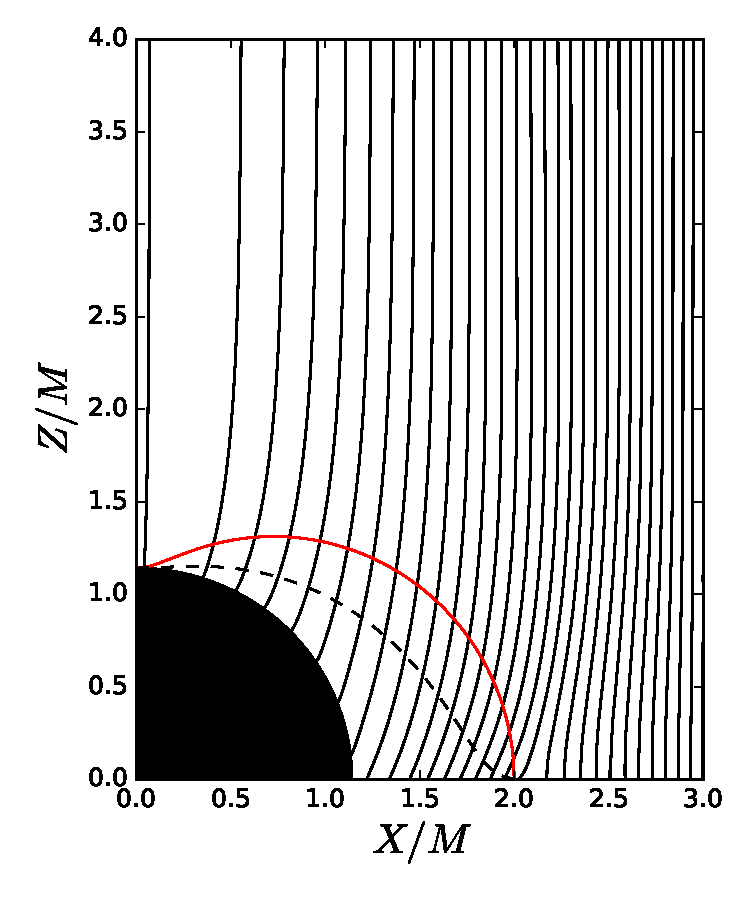
\includegraphics[scale=0.6]{f1}
\caption{\label{fig:field_lines} The configuration of field lines for the magnetosphere of a Kerr BH with spin $a=0.99$,
where the solid/red line is the ergosphere and the dashed/black line is the LS, both of which intersect with
the equator at $r=2 M$. }
\end{figure}

\begin{figure}
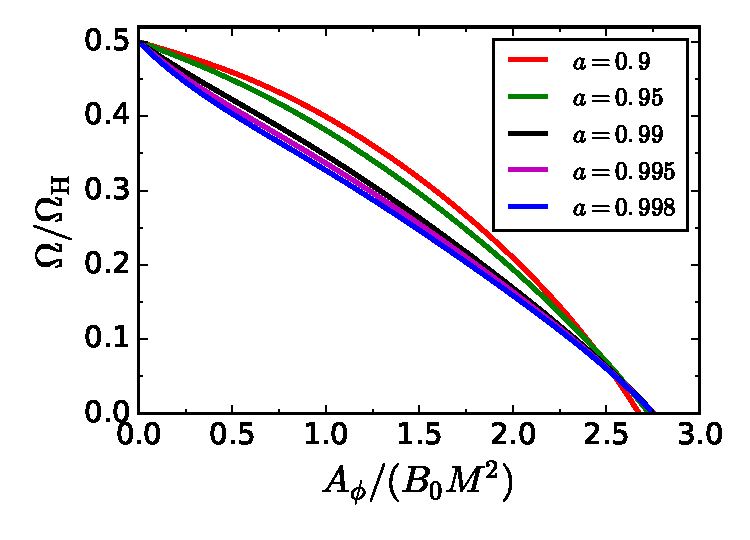
\includegraphics[scale=0.7]{f2a}
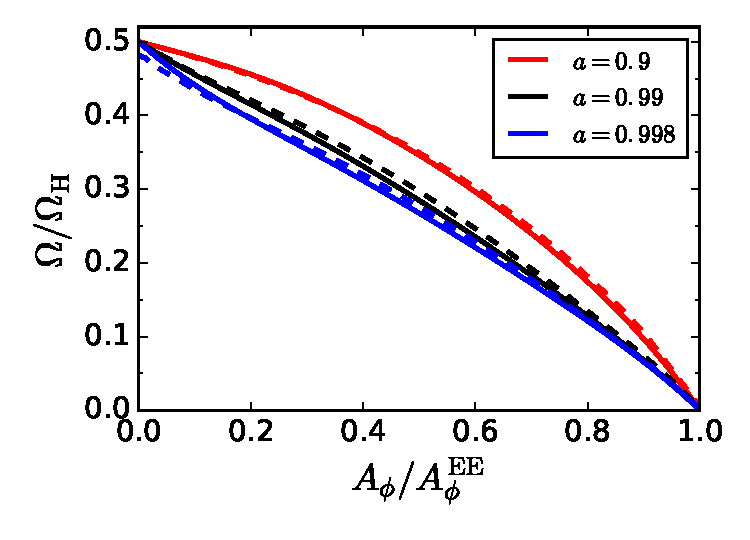
\includegraphics[scale=0.7]{f2b}
\caption{\label{fig:omega} Upper panel: the angular velocity  $\Omega(\Ap)$ for different BH spins.
Lower Panel: comparison of our numerical results (solid lines) with the simulation results of
Ref. \cite{East2018} (dashed lines). For reference, we also plot the leading order analytic solution in
dash-dotted lines.}
\end{figure}


With the angular velocity $\Omega(\Ap)$ obtained, the energy extraction rate from the BH is given by
\be
\label{eq:Edot}
\dot E = 4\pi \int_0^{\AEE} \Omega \times I \ d \Ap.
\ee
It is straightforward to obtain the energy extraction rate in the slow-rotation limit
\be
\label{eq:lowEdot}
\dot E = 128\pi \left(\frac{17}{24}-\ln 2\right) B_0^2 M^4 \WH^2.
\ee


\begin{figure}
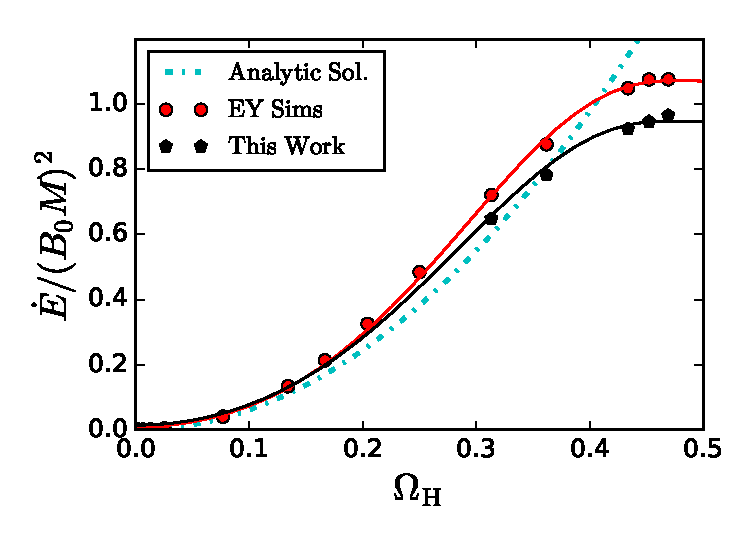
\includegraphics[scale=0.7]{f3}
\caption{\label{fig:Edot} Comparison of the energy extraction rates $\dot E(\WH)$ obtained from
three different approaches: the leading-order analytic solution (\ref{eq:lowEdot}),
our numerical solutions and  the high-resolution force-free simulations \cite{East2018}.}
\end{figure}

In Figure \ref{fig:Edot}, we compare the energy extraction rate $\dot E(\WH)$
derived from our numerical solutions with East and Yang's simulation results
\cite{East2018}, where the data points are taken from either the simulations
or our numerical solutions, while the solid lines are corresponding polynomial
fitting curves which we require to approach Eq.(\ref{eq:lowEdot}) for small
spins and to be flat for extremal spins. As expected, our energy extraction
rate $\dot E(\WH)$ is $\approx 10\%$ lower than the corresponding simulation results,
due to the $\approx 5\%$ smaller magnetic flux $\AEE$.

\section{Discussion}
\label{sec:discussion}


\subsection{Application to general field configurations}
In real astrophysical environment, we expect the field lines are more close to parabolas instead of
being strictly vertical. In many previous studies of such field
configurations \cite[e.g.][]{Tchekhovskoy2010,Nathanail2014,Mahlmann2018},
due to lacking knowledge of the equatorial boundary condition, the
equator within the ergosphere was intentionally excluded out of the computation domain by manually
introducing a ``wall" extending from the horizon-equator intersection to infinity. Such
simplification obviously misses magnetic field lines rooting on the
equatorial current sheet, which contribute about half of the total BZ flux for extremal spins in
the case of vertical field lines.

Due to the resemblance of the vertical field configuration and general parabolic field configurations,
it is natural to expect an equatorial current develops within the ergosphere,
where the magnetic dominance loses, therefore the marginally force-free boundary
condition (\ref{eq:bc3}) should also be a good work approximation here.
It is straightforward to solve the GS equation and self-consistently
impose the marginally force-free boundary condition following the
algorithm detailed in Section \ref{subsec:algorithm}.

The analysis of Section \ref{subsec:features}



\subsection{Near-horizon field configuration}
In one of our previous papers \cite{Pan2016a}, we made a claim that ``in the steady axisymmetric force-free magnetosphere
around a Kerr BH, all magnetic field lines that cross the infinite-redshift surface must intersect the event horizon".
However, simulations shows that an equatorial current sheet inevitably develops within the ergosphere , where
the force-free condition breaks down.


\section{Summary}
\label{sec:summary}

In this paper, we revisit the problem of the uniform field solution to the BZ mechanism.

\bibliography{ms}


\end{document}
